\chapter{Extended Abstract}

% ###
% Beginning of the extended abstract. We will use english in this chapter.
\selectlanguage{english}
% ###

{
\newtheorem*{abstract}{Abstract}

\begin{abstract}
    Efficient construction of the \emph{suffix array} (SA) is a still ongoing research area.
    We introduce SACABench, a benchmark system for comparing the runtime
    and memory consumption of \emph{suffix array construction algorithms} (SACAs).
    Along with this framework we include the reference implementations for many SACAs,
    parallel and sequential, as well as our own implementations.
    Although they are slower than their reference implementations in most cases,
    they can be helpful to understand the algorithms because they are written in modern C++.
    In our evaluation we compare the performance of these algorithms
    in single-threaded and multi-threaded environments.
\end{abstract}
}

\section{Introduction}

The \currentauthor{Marvin Böcker} \emph{suffix array} (\emph{\sa}) is a widely known text index,
which can be used for various string operations,
like full-text search~\cite{makinen} and construction of the Burrows-Wheeler Transform (BWT)~\cite{BWT}.
It is a permutation of all indices $1 \dots n$ of a text of length $n$ such
that the $i$th suffix of the text \inputtext has lexicographic rank $\sa[i]$.

While the efficient construction is still an active research area,
divsufsort~\cite{saca:5,saca:5:repo} is the empirically fastest
suffix array construction algorithm (SACA) since 2008\todo{wann?},
even though it has a theoretical complexity of $\mathcal O (n \log n)$,
while there are some $\mathcal O(n)$ algorithms available.

For the last year we (re-)implemented eleven SACAs~\cite{saca:3,saca:11,saca:5,saca:9,saca:1,saca:8,saca:4,saca:7,saca:10,saca:6,saca:2}
in modern C++ in order to create faster and more memory efficient implementations,
and although our attempts were mostly not successful,
we created a sophisticated benchmark framework for SACAs, \emph{\sacabench}, in the process.

In this paper we introduce \sacabench and highlight its features,
as well as document some of the optimiziation strategies we used to implement the SACAs.

\section{Benchmark Tool}

\sacabench is a CMake/C++14 project which contains many different SACAs.
There are both sequential algorithms and parallel algorithms included
and we also include the reference implementations for all of the algorithms, if one exists.
You are able to run a single, a subset of, or all of the algorithms, depending on your needs.
Time and memory consumption is automatically measured and can be output as JSON.
We also include tools to convert the JSON-format to graphs for a visual comparison of the algorithms.
Most of the graphs in this paper have been generated using SACABench directly\todo{Is that so?}.

This is the most important aspect of our framework:
the possibility to easily run many SACAs on the same input text on the same hardware
in order to measure and compare them fairly.

\subsection{Running a single algorithm}

You can evaluate a single algorithm with the command \termfont{sacabench construct} followed by the desired SACA and a path to an input file.
To get a list of all available Algorithms, you can execute the command \termfont{sacabench list}.
This will output the names for all available SACAs.
While the algorithm is running, its memory consumption is measured via the tudostat library\todo{Ist das relevant?}.
You can also enable checking of the resulting suffix array with a fast suffix array checker~\cite{saca:11} by
using the \termfont{-c} or a parrallel version with the \termfont{-q} flag.
To generate a JSON file containing detailed information about the run of the selected Algorithm separated into SACA-specific phases,
the flag \termfont{-b} needs to be added to the command, followed by a destination path to which the report will be saved to.
To override an existing file at the destination path, the option \termfont{-f} can be used.
This file can be converted to a plot on the tudostat website (see Figure \ref{tudostat_phases} as an example)\todo{Welche Abbildung ist hier gemeint?}.
If you add the flag \termfont{-{}-rplot}, a plot will be generated automatically after the SACA executed by using a R-script.
Additionally there is an alternative version of plots, which are generated using LaTex.
This can be done by adding the flag \termfont{-{}-latexplot}.
Multiple other flags and options allow to customize the way, the SACA is executed.
For example it is possible to use a prefix of the given input string by adding \termfont{-p} together with the desired prefix size. 
This enables you to use one big input file for tests with a variety of input sizes.
Also it is possibile to execute the selected SACA multiple times on the same input and to combine the results.
This can be done by using the flag \termfont{-r} followed by the number of executions.
These and many more options are listed by the tool together with an explanation by adding \termfont{-h} to any subcommand.
An example would be:

\termfont{sacabench/sacabench construct -c -b /destination/path/to/result.json -f -p 1K -r 2 -{}-rplot -{}-latexplot BPR /path/to/input}

This command executes the SACA BPR two times on a prefix of the input file of 1 KB, 
uses the checker to validate the result and writes the resulting JSON file to the given path.
If there is already a file, it would be replaced by the new file.
After the SACA finished, plots are generated with both possible options.
To reduce the number of options, you can define them in a config file in INI format.
This configuration can be used by adding the flag \termfont{-{}-config} together with the path to the file.
An example of such a configuration can be seen in \ref{sacabench-construct:config:engl}.
Using the shown file, the command 

\termfont{sacabench/sacabench construct -{}-config /path/to/config BPR /path/to/input}

is the same as the previous command.

\begin{figure}[!h]
\begin{minted}
[
frame=lines,
framesep=2mm,
baselinestretch=1.2,
fontsize=\footnotesize,
linenos,
numbersep=-4mm,
breaklines,
escapeinside=@@,
frame=single,
framesep=14pt
]
{text}
check = true
benchmark = /destination/path/to/result.json
force = true
prefix = 1K
repetitions = 2
rplot = true
latexplot = true
\end{minted}
\caption{Example for a config file for command \texttt{sacabench construct}}
\label{sacabench-construct:config:engl}
\end{figure}

\subsection{Comparing multiple algorithms}

In order to compare different SACAs with each other, you can run a set of algorithms on a given input file.
This is achieved by using the \termfont{sacabench batch} command.
Most of the options available for the command \termfont{sacabench construct} are also valid for this command.
By default all included algorithms are run, but you can either deselect certain
algorithm with the \termfont{-{}-blacklist <saca name>} flag or run only certain
algorithms by using the \termfont{-{}-whitelist <saca name>} command.
These two options can also be added to the configuration file, as seen in the previous section.
The selected algorithms are run sequentially on the input text and their memory consumption
and construction times measured.
We also supply tools to convert the resulting JSON file into several types of plots, like bar plots, strong- and weak-scaling plots.
These plots differ from the ones created by \termfont{sacabench construct}.
They put the focus on comparing multiple algorithm against each other, instead of providing detailed information about the phases of the executed SACAs.
These plots can be used to compare the algorithms fairly.

\section{SACA Overview}

There are many SACAs that operate using different principles.
The most na\"ive SACA uses a general purpose sorting algorithm to sort the suffices of the input text.
Since a string comparison is $\mathcal O (n)$ in the worst-case, this would give $\mathcal O (n^2 \log n)$ runtime.
Even though this is a sub-optimal time bound,
there are several algorithms\footnote{e.g. Deep-Shallow, mSufSort, ...} in SACABench which don't improve on this
but rather use methods to speed up the real-world performance.
These methods can be classified into the categories \emph{inducing} and \emph{doubling}:
%
\paragraph{Inducing} %
There are different methods of inducing but they mostly operate by similar principles.
When the rank of a suffix $i$ (that is the position of $i$ in the SA) is known,
it is possible to deduce the rank of other suffixes $j$.

The easiest to understand usecase for this is when using buckets.
Recall that a bucket $\mathsf b_{\sigma}$ is a region of the suffix
array which contains only and all the suffixes,
which start with the substring $\sigma$.
It is obvious that all the subbuckets $\mathsf b_{\sigma\alpha}$ for
every $\alpha \in \Sigma$ are contained within $\mathsf b_\sigma$.
It is possible to \emph{induce} the order of the $\mathsf b_{\alpha\sigma}$ bucket,
if all Buckets $\mathsf b_\sigma$ for every possible $\sigma \in \Sigma$ are already sorted (by whatever method),
since you know the regions of $\mathsf b_\alpha$ that are the $\mathsf b_{\alpha\sigma}$ Subbuckets.
You can then (for $\sigma \in \Sigma$) find the suffixes of $\mathsf b_{\alpha\sigma}$ in $\mathsf b_{\sigma}$,
subtract one of every index and write the found suffixes in-order to $\mathsf b_{\alpha\sigma}$.
Since the suffixes of $\mathsf b_{\alpha\sigma}$ are essentially the same as $\mathsf b_\sigma$ but
with only one (the same) character added in front of them,
their relative ordering is the same as the suffixes in $\mathsf b_\sigma$.
This method is used in e.g. Deep-Shallow~\cite{saca:4} and 
Bucket Pointer Refinement~\cite{saca:2}\todo{more sacas? correct refs?}.

Another method of induction relies on the property of L- and S-Type suffixes and
is most prominently used in the SAIS-Algorithm.
This algorihm is based on the sorting of all the LMS suffixes (by recursion)
and a Left-to-right-pass (to induce the L suffixes)
and a Right-to-left-pass (to induce the S suffixes)\todo{nachschlagen wir der sais ging}.
It can be shown that after these two passes the resulting suffix array is correct.

\paragraph{Doubling} Another fundamentally different approach to suffix sorting
aims to double the length of sorted suffixes in every iteration.
This is done by first sorting the suffixes by their first character only.
To then deduce the ordering of all the elements in the $\mathsf b_\alpha$ bucket,
one can look at the relative ordering of the suffixes that start one position
after the to-be-sorted suffix:
their relative ordering decide the ordering of the original suffixes.
In the next iteration one can look at the suffixes that start two positions later in the text,
and so on.
After $\mathcal O(\log n)$ iterations (since we double the prefix size in every iteration),
all the suffixes are sorted.
This method is used by qsufsort~\cite{unknown}\todo{fix ref} and the
doubling/discarding algorithm originally developed for use with external memory~\cite{saca:11}.

\bigskip

There are also some recursive algorithms, which mostly operate on a shared principle:
%
\paragraph{Recursive} Some algorithms, such as DC3~\cite{xxx} and SAIS~\cite{xxx}\todo{ref?} require to sort a
partial set of suffixes as part of their task to sort the entire suffix array.
As they are able to do this by calling themselves with a different input, they are called \emph{recursive algorithms}.
DC3 sorts exactly $^2\!/\!_3$ of the suffixes by recursion, while SAIS sorts all the LMS suffices by recursion,
if their ordering cannot be decided by looking at their first character.
After this step, the ordering of the other suffixes can be induced.

\begin{figure}[!t]
    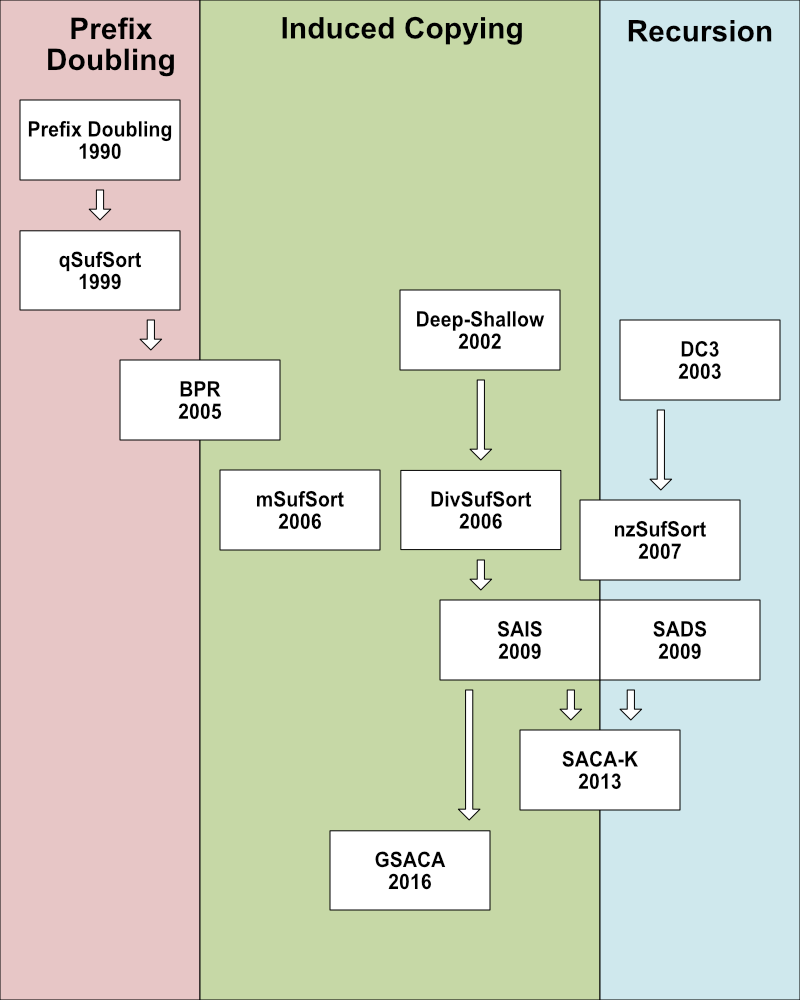
\includegraphics[width=\textwidth]{kapitel/5_saca_uebersicht/history/history3_eng.png}
    \caption{(partial) History of SACAs}
    \label{ea:fig:history}
\end{figure}

See Figure \ref{ea:fig:history} for a short summary of SACA history.
The different SACAs are divided into the three classes described above.
We now briefly explain the shown algorithms and their differences.

Prefix Doubling is a SACA which works purely by the above described method \emph{Doubling}.
In every iteration the SA is refined and double the amount of characters are considered for sorting.
This directly influenced qsufsort, which improved its performance~\cite{hermann?}.
BPR incorporated some ideas of inducing with prefix doubling and is therefore on the edge of those two paradigms.
Its inducing is based on the copy-technique by Seward~\cite{seward2000}\todo{right ref?}.
This technique is also used by Deep-Shallow, which uses string-sorting instead of prefix doubling.
It influenced divsufsort, which \todo{Olli? Adde hier mal shit}.
mSufSort is another inducing-SACA, but since it constructs the \emph{inverse suffix array} instead of the SA,
it's not derived from any other SACA.
SAIS/SADS take inducing one step further than DivSufSort and induce most suffixes after a recursion step.
This is also done by SACA-K and GSACA, which are both similar to SAIS, but add some optimizations
(SACA-K for example doesn't use any extra space).
The two other recursive SACAs are DC3 (which sorts $\frac{2}{3}$ of the suffixes in a recursion step)
and nzSufSort (which is similar to DC3 but improves on some aspects)\todo{nico? johannes? bitte ergänzen}.

\section{Optimization Strategies}

As with most programs, much of the performance of SACAs is dependent on efficiently implementing these algorithms.
We therefore used some practical optimizations to the descriptions of the algorithms to improve performance.
The following is an incomplete list of tricks one can use to do so.

\subsection{Different bit lengths for the suffix array}

We implemented our SACAs with an exchangable suffix array index type, that is a different bit length for the indices in the suffix array.
With our current implementation it is possible to use 32, 40, 48 and 64 bit for the suffix array elements.
Since our tool supports a different output encoding (32 or 64 bit), we can save memory during construction regardless of the desired output length.
Keep in mind that since the 40- and 48-bit types are not standardized, their performance is inferior to those of 32- and 64- bit types.
We measured an approximate 2.5x slowdown compared to the built-in number types.\todo{Nochmal richtig messen?}

\subsection{Cache-efficiency}

The most crucial part of optimizing a SACA is cache-efficiency, that is aiming for time-local and space-local memory access.
Since the SA is a pseudo-random mutation of numbers, the SA can't be written cache-efficiently.
However, when implementing SACAs, avoiding unnecessary cache misses can significantly improve performance.

\subsection{Wordpacking}

To maximize throughput, multiple characters of the input (8 bit each) can be processed as a whole by
interpreting them as integer numbers (64 bit, or even up to 512 bit by using vector operations).
Algorithms using wordpacking techniques are the Osipov algorithm \todo{Referenz}, Doubling \todo{Referenz}, Discarding \todo{Referenz} and QSufSort \todo{Referenz}.

\subsection{Sorting Algorithms}

Many SACAs use sorting algorithms at some point, so for the benchmark a variety of sorting algorithms were implemented so that all SACAs can use them. Included are some versions of quicksort, bucketsort and versions of radixsort.  This is especially interesting for naive parallelization, where one may just switch from a sequential sorting algorithm to a parallel one and thereby improve performance.
Besides our own implemented sorting algorithms some external sorting algorithms are also included. Most of those external sorting algorithms are made for parallel use.

\subsubsection{Binary vs. ternary comparison-based sort}

Multiple versions of quicksort are implemented:
Two of them are introsort~\cite{Musser97} and ternary quicksort~\cite{ternary_quicksort}.
It has been shown that the binary sorting procedure is faster,
if there are no equal elements in the set to be sorted \todo{Graph oder Messung?};
else, the ternary version is faster~\cite{ternary_quicksort}.
We therefore chose the best option for the required use-case.

\section{Evaluation}



\section{Conclusion}

We introduced SACABench, an extensive framework for benchmarking and comparing suffix array construction algorithms.
It includes a large set of publicly available SACAs and simplifies the comparison of these with new SACAs.
The code is written in modern C++ and well documented and can therefore be helpful in understanding the algorithms.
We also include several parallel SACAs as well as parallel reference implementations.

In our evaluation we confirmed divsufsorts dominance on most of the tested texts.

% ###
% End of extended abstract, switch language to german again
\selectlanguage{ngerman}
% ###
